\section{Least Squares}\label{sec:least-squares}

Many problems in autonomous driving can be written as: \emph{find the parameters that best explain a set of noisy measurements}.
Fitting a line to some points, estimating the pose of a camera, calibrating a sensor or fusing several measurements are all instances of the same problem, and the standard tool to solve it is \textbf{least squares}.

Least squares is used for:
\begin{compactitemize}
    \item \textbf{data fitting}: find the curve or line that best approximates a set of measurements;
    \item \textbf{regression analysis}: estimate the relationships between variables (e.g.\ linear regression);
    \item \textbf{parameter estimation}: identify the unknown parameters of physical and mathematical models;
    \item \textbf{signal processing}: denoise signals or estimate system responses;
    \item \textbf{machine learning}: it is the basis of many supervised learning methods;
    \item \textbf{control and robotics}: state estimation, sensor fusion and trajectory fitting.
\end{compactitemize}

\subsection{Linear least squares}
Consider an \textbf{overdetermined} linear system, i.e.\ a system with more equations than unknowns:
\[
\underbrace{A}_{m\times n}\ x \;\approx\; \underbrace{b}_{m\times1}, \qquad m > n
\]
Each equation is a constraint on the unknown $x$ but, because of noise and inconsistencies, a solution that satisfies all the equations exactly may not exist.

The \textbf{least squares principle} says: find the estimate $\hat{x}$ that minimizes the \textbf{total squared error} over all the equations,
\[
\hat{x} = \arg\min_x \|Ax - b\|_2^2 = \arg\min_x \sum_{i=1}^{m} \left(a_i^T x - b_i\right)^2
\]
where $a_i^T$ is the $i$-th row of $A$.
Each equation contributes a \textbf{residual}
\[
r_i = a_i^T \hat{x} - b_i
\]
and the solution balances the residuals so that their sum of squares is minimal.
The single equations are not necessarily satisfied: their residuals do not need to be zero.

\subsubsection{Normal equations}
To find the minimum, we expand the error:
\[
\|Ax - b\|_2^2 = (Ax - b)^T (Ax - b) = x^T A^T A\, x - 2\, x^T A^T b + b^T b
\]
and we set its derivative with respect to $x$ to zero:
\[
\frac{d}{dx}\left( x^T A^T A\, x - 2\, x^T A^T b + b^T b \right) = 2A^T A\, x - 2A^T b = 0
\]
This gives the \textbf{normal equations}:
\[
A^T A\, x = A^T b \qquad\Longleftrightarrow\qquad H x = g
\]
where $H = A^T A$ is (up to a factor 2) the \textbf{Hessian} of $\|Ax - b\|_2^2$, and $g = A^T b$ is related to its \textbf{gradient}.
Solving them for $x$:
\[
\hat{x} = (A^T A)^{-1} A^T b
\]
In practice we do not compute the inverse explicitly, but use a matrix decomposition. With the SVD of $A^T A = U \Sigma V^T$:
\[
\hat{x} = V\, \Sigma^{-1} U^T A^T b
\]

\begin{infobox}[Reminder: Singular Value Decomposition (SVD)]
Any real matrix $A \in \mathbb{R}^{m\times n}$ can be decomposed as
\[
A = U\, \Sigma\, V^T
\]
where $U \in \mathbb{R}^{m\times m}$ is orthogonal (left singular vectors), $\Sigma \in \mathbb{R}^{m\times n}$ is diagonal with the non-negative singular values, and $V \in \mathbb{R}^{n\times n}$ is orthogonal (right singular vectors).
Geometrically, $A$ does: rotate ($V^T$) $\rightarrow$ stretch ($\Sigma$) $\rightarrow$ rotate ($U$).
It is used to compute pseudoinverses (least squares solutions), for dimensionality reduction (PCA), noise reduction and data compression.
\end{infobox}

\subsubsection{Evaluating the fit: RMSE}
After fitting a model, we need to quantify how well it explains the observations.
The \textbf{Root Mean Squared Error} (RMSE) measures the average magnitude of the residuals:
\[
\mathrm{RMSE} = \sqrt{\frac{1}{N} \sum_{i=1}^{N} \left(y_i - \hat{y}_i\right)^2} = \sqrt{\frac{1}{N} \sum_{i=1}^{N} \left(y_i - f(x_i)\right)^2}
\]
where $y_i$ are the observed data, $\hat{y}_i = f(x_i)$ the predictions of the fitted model and $N$ the number of observations.
The RMSE is always non-negative, and a lower RMSE means a better fit.

\begin{figure}[H]
    \centering
    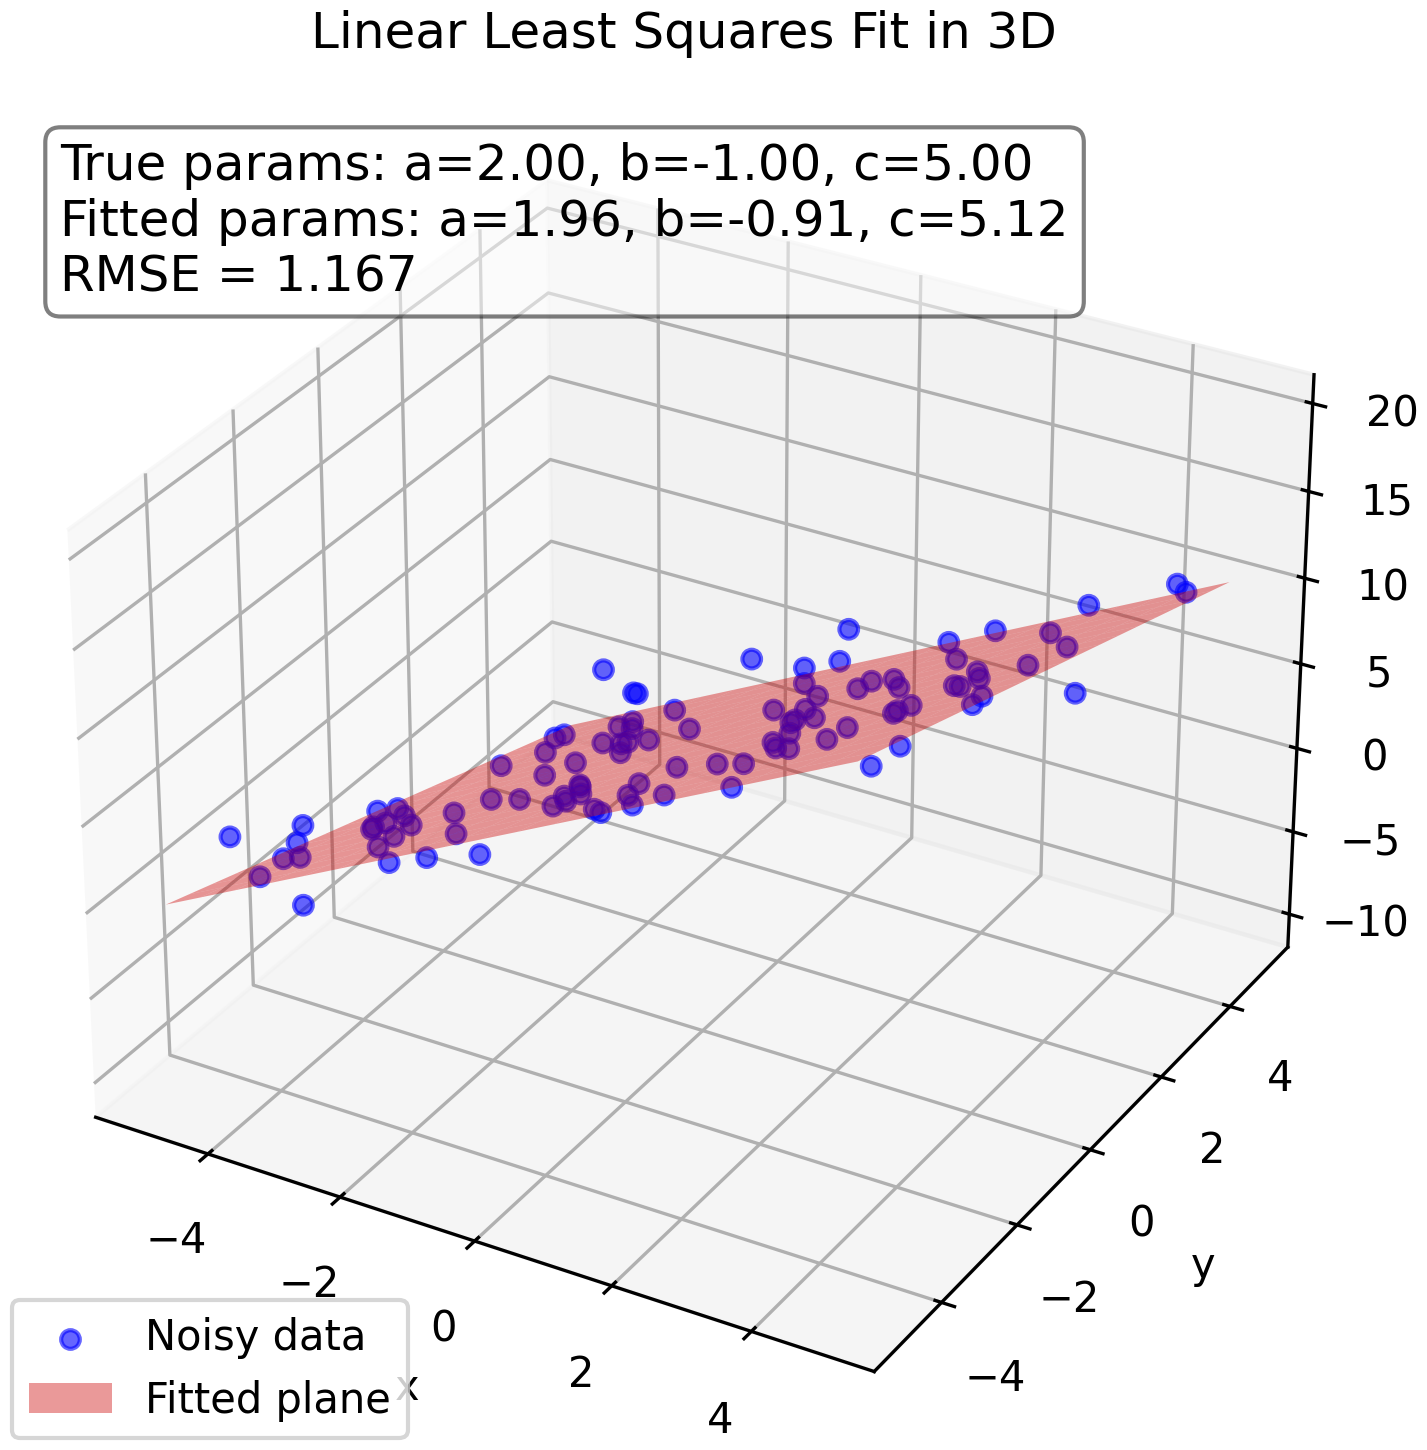
\includegraphics[width=0.5\textwidth]{images/C9_1.png}
    \caption{Least squares fit of a plane $z = ax + by + c$ to noisy 3D points}
\end{figure}

\begin{infobox}[Decomposing the RMSE: bias and variance]
The RMSE is a single number, so it tells us \emph{how much} we are wrong but not \emph{why}. To understand the cause, we can split it into two parts. We call $e_i = y_i - \hat{y}_i$ the error on the $i$-th sample and we define two quantities.

The \textbf{bias} is the actual mean of the error:
\[
\mu_e = \frac{1}{N}\sum_{i=1}^{N} e_i
\]
It is a \emph{systematic} error. If $\mu_e \neq 0$, the estimates are always shifted in the same direction, for example always too long or always too far to the left. Collecting more data does not make it go away, because every new sample carries the same offset.

The \textbf{variance} measures how much the errors are spread around their mean:
\[
\sigma_e^2 = \frac{1}{N}\sum_{i=1}^{N} \left(e_i - \mu_e\right)^2
\]
It is the \emph{random} part of the error, and it tells us how confident we can be about the mean. A small variance means that the errors are all very close to $\mu_e$, so the behaviour is repeatable and predictable. A large variance means that the single errors jump around a lot. Even if they average to the right value, each single estimate cannot be trusted much.

Expanding the square $e_i^2 = \left((e_i - \mu_e) + \mu_e\right)^2$ splits the sum into three terms. The mixed term $2\mu_e\sum_i (e_i-\mu_e)$ is zero by the definition of $\mu_e$, so we get:
\[
\mathrm{MSE} = \frac{1}{N}\sum_{i=1}^{N} e_i^2 = \mu_e^2 + \sigma_e^2
\qquad\Longrightarrow\qquad
\boxed{\mathrm{RMSE} = \sqrt{\mu_e^2 + \sigma_e^2}}
\]

\textbf{Practical consequence.} When the RMSE is high, we should not just conclude that the system is bad. We should compute bias and variance separately and find the \emph{culprit}, because the two problems have very different fixes:
\begin{itemize}
    \item \textbf{High bias}: something is systematically wrong. Typical causes are a wrong calibration (intrinsic or extrinsic), a wrong model, a wrong reference frame or a time offset between sensors. We fix it by calibrating or by correcting the model. Once the bias is known, it can even be subtracted directly.
    \item \textbf{High variance}: the measurements are noisy. Typical causes are sensor noise, vibrations or outliers. We fix it by filtering (e.g.\ a Kalman filter), by averaging more measurements, by using robust weights (IRLS) or by using a better sensor.
\end{itemize}
\end{infobox}

\begin{examplebox}[Finding the culprit: two LiDARs]
A vehicle is parked $10\,\mathrm{m}$ in front of a wall, and we measure this distance $N$ times with two different LiDARs. Both give the \emph{same} RMSE of $0.5\,\mathrm{m}$, but for very different reasons.

\textbf{LiDAR A:} $\mu_e = 0.48\,\mathrm{m}$ and $\sigma_e = 0.14\,\mathrm{m}$, so
\[
\mathrm{RMSE}_A = \sqrt{0.48^2 + 0.14^2} = \sqrt{0.2304 + 0.0196} = 0.5\,\mathrm{m}
\]
Almost all of the error comes from the bias. The sensor always measures about $10.48\,\mathrm{m}$, and it is very repeatable. This is the typical sign of a \textbf{calibration problem}, for example a wrong extrinsic translation between the LiDAR and the vehicle frame. If we estimate the offset and correct it, the RMSE drops to about $0.14\,\mathrm{m}$, and no filtering is needed.

\textbf{LiDAR B:} $\mu_e = 0$ and $\sigma_e = 0.5\,\mathrm{m}$, so
\[
\mathrm{RMSE}_B = \sqrt{0^2 + 0.5^2} = 0.5\,\mathrm{m}
\]
Here the sensor is correct \emph{on average}, but every single measurement can be off by half a metre. Calibrating does not help, because there is no offset to remove. We need to reduce the \textbf{noise}, for example by averaging several scans, filtering over time with a Kalman filter, or using a less noisy sensor.

\begin{center}
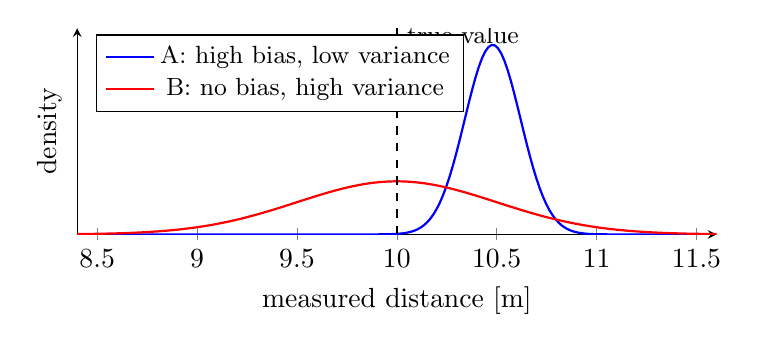
\begin{tikzpicture}
\begin{axis}[
    width=0.8\linewidth, height=4.2cm,
    axis lines=left,
    xlabel={measured distance [m]}, ylabel={density},
    xmin=8.4, xmax=11.6, ymin=0, ymax=3.1,
    ytick=\empty,
    samples=200,
    legend pos=north west, legend style={font=\small},
]
\addplot[blue, thick, domain=8.4:11.6] {1/(0.14*sqrt(2*pi))*exp(-(x-10.48)^2/(2*0.14^2))};
\addlegendentry{A: high bias, low variance}
\addplot[red, thick, domain=8.4:11.6] {1/(0.5*sqrt(2*pi))*exp(-(x-10)^2/(2*0.5^2))};
\addlegendentry{B: no bias, high variance}
\draw[dashed, thick] (axis cs:10,0) -- (axis cs:10,3.1) node[pos=0.97, right, font=\small] {true value};
\end{axis}
\end{tikzpicture}
\end{center}
So two sensors with the same RMSE can need completely opposite fixes. Looking only at the RMSE would not tell us which one to apply.
\end{examplebox}

\subsection{Weighted least squares}
Standard least squares assumes that all the measurements are equally important. Often, however, they have a different \textbf{reliability} (e.g.\ different variances).
In \textbf{Weighted Least Squares} (WLS) we assign a weight $w_i > 0$ to each observation:
\[
\min_x \sum_{i=1}^{N} w_i \left(y_i - a_i^T x\right)^2
\]
In matrix form, with $W = \mathrm{diag}(w_1, \dots, w_N)$:
\[
\min_x\ (Ax - b)^T\, W\, (Ax - b)
\]
and the solution is:
\[
\hat{x} = (A^T W A)^{-1} A^T W b
\]
A natural choice is $w_i = 1/\sigma_i^2$: the more precise a measurement, the more it counts (exactly as in the Kalman filter).

\begin{figure}[H]
    \centering
    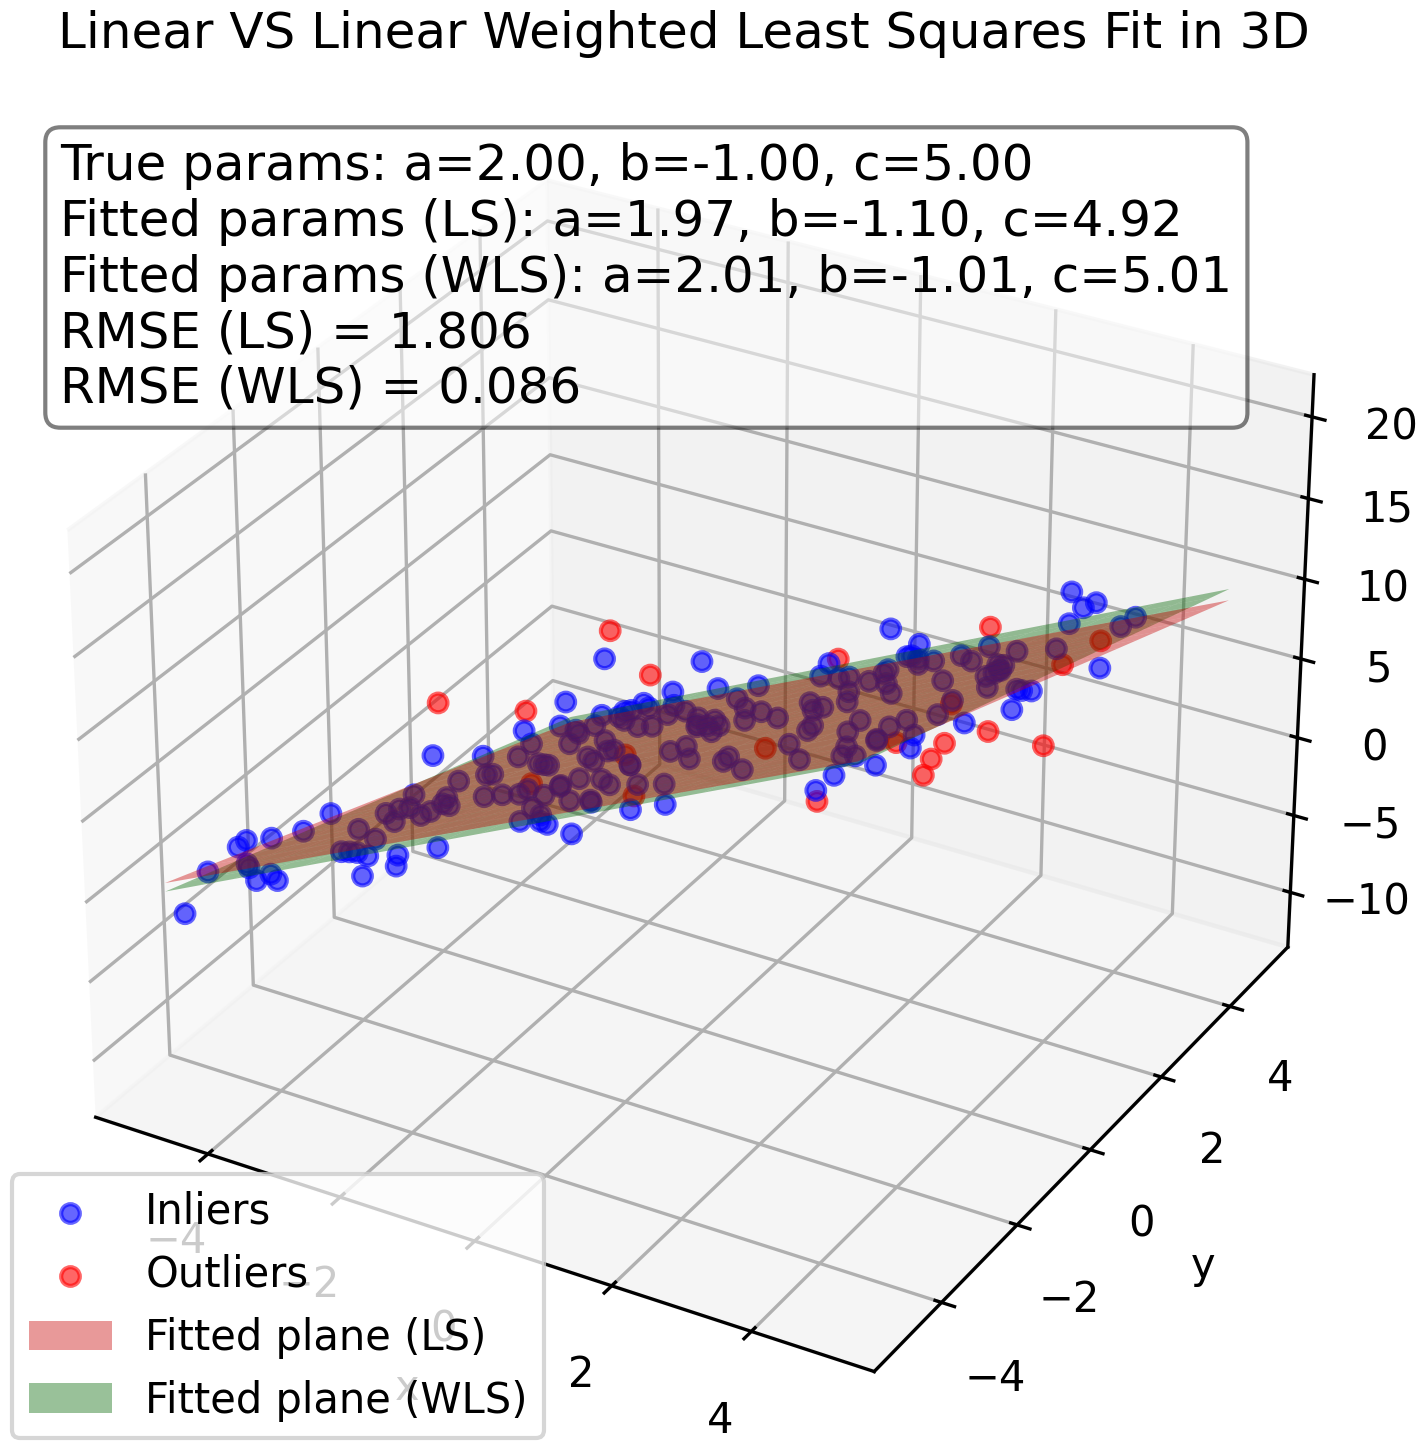
\includegraphics[width=0.5\textwidth]{images/C9_2.png}
    \caption{With outliers (red), plain least squares (LS) is pulled away, while weighted least squares (WLS) fits the inliers}
\end{figure}

\subsection{Iterative reweighted least squares (IRLS)}
Standard least squares is \textbf{sensitive to outliers}: since the residuals are squared, a single point far from the others has a huge influence on the result.
\textbf{IRLS} reduces their influence by adapting the weights at each iteration:
\begin{enumerate}
    \item start with an initial estimate $x^{(0)}$ (e.g.\ the linear least squares solution);
    \item at each iteration $k$, compute the residuals:
    \[
    r_i^{(k)} = y_i - a_i^T x^{(k)}
    \]
    \item define the weights as a function of the residuals, $w_i^{(k)} = f\big(r_i^{(k)}\big)$, giving smaller weights to large residuals;
    \item solve the weighted least squares problem:
    \[
    x^{(k+1)} = \arg\min_x \sum_i w_i^{(k)} \left(y_i - a_i^T x\right)^2
    \]
    \item repeat until convergence.
\end{enumerate}

\subsubsection{Weight functions}
Common weight functions are ($c$ is a parameter that scales the effect of the function):

\textbf{Huber}:
\[
w(r) = \begin{cases} 1 & |r| \le c \\[2pt] \dfrac{c}{|r|} & |r| > c \end{cases}
\]

\textbf{Cauchy}:
\[
w(r) = \frac{1}{1 + \left(\frac{r}{c}\right)^2}
\]

\textbf{Tukey's biweight}:
\[
w(r) = \begin{cases} \left(1 - \left(\frac{r}{c}\right)^2\right)^2 & |r| \le c \\[2pt] 0 & |r| > c \end{cases}
\]

\textbf{L1} (absolute loss):
\[
w(r) = \frac{1}{|r|}
\]

The intuition is always the same: \textbf{large residuals $\Rightarrow$ smaller weights $\Rightarrow$ reduced influence of the outliers}.
Huber keeps the points close to the model with full weight, Cauchy reduces the weight smoothly, while Tukey completely ignores the points beyond $c$.

\begin{figure}[H]
    \centering
    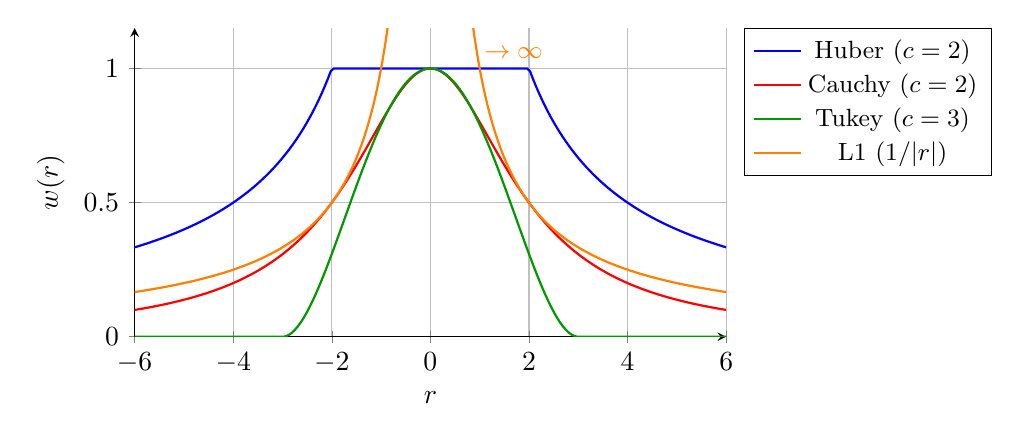
\begin{tikzpicture}
        \begin{axis}[
            width=0.75\textwidth, height=5.5cm,
            xmin=-6, xmax=6, ymin=0, ymax=1.15,
            xlabel={$r$}, ylabel={$w(r)$},
            axis lines=left, legend pos=outer north east, grid=major,
            legend style={font=\small}, samples=200, domain=-6:6]
            \addplot[blue, thick] {abs(x)<=2 ? 1 : 2/abs(x)};
            \addlegendentry{Huber ($c=2$)}
            \addplot[red, thick] {1/(1+(x/2)^2)};
            \addlegendentry{Cauchy ($c=2$)}
            \addplot[green!60!black, thick] {abs(x)<=3 ? (1-(x/3)^2)^2 : 0};
            \addlegendentry{Tukey ($c=3$)}
            \addplot[orange, thick, domain=-6:-0.2, samples=400, forget plot] {1/abs(x)};
            \addplot[orange, thick, domain=0.2:6, samples=400] {1/abs(x)};
            \node[orange, font=\small, anchor=south west] at (axis cs:0.9,1.0) {$\to\infty$};
            \addlegendentry{L1 ($1/|r|$)}
        \end{axis}
    \end{tikzpicture}
    \caption{Weight functions used in IRLS}
\end{figure}

\begin{figure}[H]
    \centering
    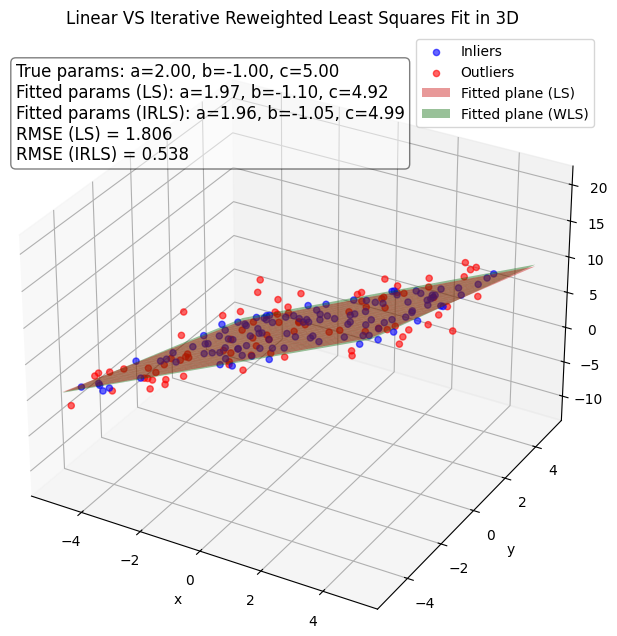
\includegraphics[width=0.5\textwidth]{images/C9_3.png}
    \caption{Least squares vs iterative reweighted least squares with outliers}
\end{figure}

\subsection{Non-linear least squares (NLLS)}
Often the model is \textbf{not linear} in the parameters (e.g.\ a camera projection, which contains rotations and a division by the depth).
The goal of \textbf{non-linear least squares} is to fit a non-linear model to the data by minimizing the sum of squared residuals:
\[
\min_\theta \sum_{i=1}^{n} \left\| y_i - f(x_i; \theta) \right\|_2^2 = \min_\theta \sum_{i=1}^{n} \left\| r_i(\theta) \right\|_2^2
\]
where $x_i$ are the input data, $y_i$ the observed outputs, $f(x_i; \theta)$ the non-linear model with parameters $\theta \in \mathbb{R}^D$,
\[
r_i(\theta) = y_i - f(x_i; \theta)
\]
is the \textbf{residual}, and $\sum_i \|r_i(\theta)\|_2^2$ is the \textbf{cost function}.
There is \textbf{no closed-form solution}: we need an iterative approach.

\subsubsection{Gauss--Newton algorithm}
The \textbf{Gauss--Newton} algorithm solves NLLS by repeatedly linearizing the problem:
\begin{enumerate}
    \item start with an initial guess $\theta_0$;
    \item use a first-order Taylor expansion of the residuals around the current solution $\theta_k$, where $J_{r_i}$ is the Jacobian of $r_i$:
    \[
    \min_\theta \sum_{i=1}^{n} \|r_i(\theta)\|_2^2 \;\approx\; \min_{\Delta\theta} \sum_{i=1}^{n} \left\| r_i(\theta_k) + J_{r_i}(\theta_k)\, \Delta\theta \right\|_2^2
    \]
    \item the cost is now a \textbf{linear least squares} problem in $\Delta\theta$, of the form $\|Ax - b\|_2^2$:
    \[
    \left\| \begin{bmatrix} J_{r_1}^T \\ \vdots \\ J_{r_n}^T \end{bmatrix} \Delta\theta - \begin{bmatrix} -r_1(\theta_k) \\ \vdots \\ -r_n(\theta_k) \end{bmatrix} \right\|_2^2 = \left\| J_r\, \Delta\theta - r \right\|_2^2
    \]
    so, from the normal equations,
    \[
    \Delta\theta = (J_r^T J_r)^{-1} J_r^T\, r = -H^{-1} g
    \]
    \item update the parameters:
    \[
    \theta_{k+1} = \theta_k - \Delta\theta
    \]
    \item go back to step 2 until convergence, or until the maximum number of iterations is reached.
\end{enumerate}

\subsubsection{Line search and trust region}
Unfortunately, naively solving a sequence of these linear problems and updating $\theta$ may \textbf{not converge}: the linearization is valid only close to $\theta_k$, and a too large step can increase the cost.
To get a convergent algorithm we need to \textbf{control the size of the step}, and there are two families of methods:
\begin{compactitemize}
    \item \textbf{Line search}: first find a \textbf{descent direction} along which the cost decreases, then compute a \textbf{step size} that decides how far to move along it;
    \item \textbf{Trust region}: approximate the cost function only inside a region around the current point (the \textbf{trust region}). If the approximation succeeds in decreasing the true cost, the region is \textbf{expanded}; otherwise it is \textbf{contracted} and the problem is solved again.
\end{compactitemize}

\begin{figure}[H]
    \centering
    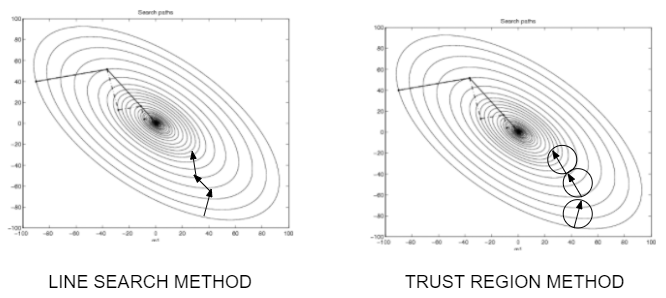
\includegraphics[width=0.6\textwidth]{images/C9_4.png}
    \caption{Line search (left) vs trust region (right)}
\end{figure}

\subsubsection{Levenberg--Marquardt algorithm}
\textbf{Levenberg--Marquardt} (LM) is the most popular trust region algorithm for NLLS. At each iteration it solves:
\[
\min_{\Delta\theta}\ \left\| J_r\, \Delta\theta - r \right\|_2^2 + \frac{1}{\mu} \left\| D\, \Delta\theta \right\|_2^2
\]
where:
\begin{compactitemize}
    \item $\mu$ is the \textbf{trust region radius}: the larger it is, the more we trust the linear approximation, and the less the second term affects the total cost (LM behaves like Gauss--Newton); the smaller it is, the more the step is penalized and kept short;
    \item $D$ is a diagonal matrix, typically the square root of the diagonal of $J_r^T J_r$. These diagonal entries measure how strongly each parameter influences the cost: a large value means that the cost is very sensitive to that parameter, so its variation should be limited more, because the linear approximation may not describe well how the function changes.
\end{compactitemize}

The LM problem is still a \textbf{linear least squares} problem, since we can stack the two terms:
\[
J' = \begin{bmatrix} J_r \\ \frac{1}{\sqrt{\mu}}\, D \end{bmatrix}, \qquad b' = \begin{bmatrix} r \\ 0 \end{bmatrix}
\]
and solve:
\[
\min_{\Delta\theta} \left\| J'\, \Delta\theta - b' \right\|_2^2
\]

\subsection{Solving NLLS efficiently}
\subsubsection{Computational cost}
In each iteration of Levenberg--Marquardt, the dominant cost is solving the linear system for $\Delta\theta$, which requires \textbf{factorizing} $J_r$ or $J_r^T J_r$.
In general, factorizing an $m \times n$ matrix costs
\[
O(m\, n^2)
\]
and $J_r$ is $m \times n$, where $m$ is the total number of \textbf{residuals} and $n$ the total number of \textbf{parameters}.
So the cost of solving an NLLS problem grows with the number of residuals and, much faster, with the number of parameters to estimate.

\subsubsection{Matrix factorizations}
For small problems we can solve the linear system with the SVD, as in the linear case. When the system becomes large, however, the SVD is \textbf{no longer sustainable}, because it is too expensive in time and memory. We therefore use cheaper factorizations, mainly QR and Cholesky.

Both methods start from the solution of the normal equations:
\[
\Delta\theta = (J_r^T J_r)^{-1} J_r^T\, r
\]
and use two properties of the inverse and transpose of a product:
\[
(AB)^{-1} = B^{-1}A^{-1}, \qquad (AB)^T = B^T A^T, \qquad (A^T)^{-1} = (A^{-1})^T \eqqcolon A^{-T}
\]

\subparagraph{QR decomposition.} We factorize the Jacobian itself as
\[
J_r = QR
\]
where $Q$ ($m\times n$) has orthonormal columns, so $Q^T Q = I$, and $R$ ($n\times n$) is upper triangular. If $J_r$ has full rank, $R$ is invertible. Step by step:
\begin{enumerate}
    \item Product $J_r^T J_r$:
    \[
    J_r^T J_r = (QR)^T (QR) = R^T Q^T Q R = R^T I R = R^T R
    \]
    \item Its inverse:
    \[
    (J_r^T J_r)^{-1} = (R^T R)^{-1} = R^{-1} (R^T)^{-1} = R^{-1} R^{-T}
    \]
    \item The term $J_r^T r$:
    \[
    J_r^T r = (QR)^T r = R^T Q^T r
    \]
    \item Putting everything together, $R^{-T} R^T = I$ simplifies:
    \[
    \Delta\theta = R^{-1} \underbrace{R^{-T} R^T}_{I} Q^T r = R^{-1} Q^T r
    \]
\end{enumerate}
In practice $R^{-1}$ is never computed explicitly. We solve the triangular system
\[
R\, \Delta\theta = Q^T r
\]
by \textbf{back substitution}, starting from the last unknown, at a cost of only $O(n^2)$.

\subparagraph{Cholesky decomposition.} Here we factorize the small $n\times n$ matrix of the normal equations:
\[
J_r^T J_r = L^T L
\]
where $L$ is upper triangular, so $L^T$ is lower triangular. Step by step:
\begin{enumerate}
    \item We form the matrix $J_r^T J_r$ and the vector $J_r^T r$.
    \item We compute the factorization $J_r^T J_r = L^T L$.
    \item We invert the product:
    \[
    (J_r^T J_r)^{-1} = (L^T L)^{-1} = L^{-1} (L^T)^{-1} = L^{-1} L^{-T}
    \]
    \item We substitute it in the solution:
    \[
    \Delta\theta = L^{-1} L^{-T} J_r^T\, r
    \]
\end{enumerate}
Again, no inverse is computed in practice. We write the normal equations as $L^T L\,\Delta\theta = J_r^T r$, call $y = L\,\Delta\theta$, and solve two triangular systems:
\[
L^T y = J_r^T r \quad \text{(forward substitution)}, \qquad L\, \Delta\theta = y \quad \text{(back substitution)}
\]

Comparing step 1 of the QR derivation with the Cholesky factorization, we find $J_r^T J_r = R^T R = L^T L$. So the $R$ of the QR decomposition is exactly the Cholesky factor $L$, up to the signs of its rows. The two methods compute the same triangular matrix, but QR gets it directly from $J_r$, while Cholesky gets it from $J_r^T J_r$.

The Jacobian usually has many more rows than columns. Since the cost of QR grows linearly with the number of rows, beyond a certain size \textbf{Cholesky} is more efficient (it works on the small $n\times n$ matrix $J_r^T J_r$).
On the other hand, Cholesky is \textbf{numerically less stable}, and it may fail for ill-conditioned Jacobians.

The standard Cholesky decomposition only works if the matrix $J_r^T J_r$ is symmetric and \textbf{positive definite}. In theory $J_r^T J_r$ is always at least positive semi-definite, because
\[
x^T J_r^T J_r\, x = \lVert J_r x \rVert^2 \ge 0 \quad \forall x
\]
In practice, however, it can be singular or almost singular. This happens when some parameters are not observable (rank-deficient Jacobian), when the problem is ill-conditioned, or because of round-off errors. In that case the factorization breaks down (for example it tries to take the square root of a negative number), and the computed step $\Delta\theta$ is \textbf{wrong}.

For this reason there are \textbf{modified Cholesky} decompositions. They detect during the factorization that the matrix is not positive definite, and they apply \textbf{heuristics} to make it positive definite, typically by adding a small positive term to the diagonal. This makes the method robust, but it is also \textbf{computationally heavier} than the standard version.

\subsubsection{Sparse Jacobians}
Even QR and Cholesky are not efficient enough for very large matrices, so we need further tricks. The most important one is to exploit the structure of the Jacobian.

In large NLLS problems the Jacobian is usually \textbf{sparse}: each residual depends only on a few parameters, so most entries are zero. Often \textbf{80\% or more} of the matrix is made of zeros.
For example, in SLAM or bundle adjustment each residual is the observation of one landmark from one pose. Its row of the Jacobian is therefore non-zero only in the columns of that pose and of that landmark, and it is zero everywhere else.
Dense QR or Cholesky factorizations are inefficient in this case, and it is better to use routines that treat the Jacobian as a sparse matrix and compute a sparse factor, such as \textbf{sparse Cholesky} or the \textbf{sparse Schur complement}.
This leads to substantial savings in memory and CPU time.

\subsection{Robust NLLS}
NLLS can be made \textbf{robust to outliers} in the same way as the linear case, either with a \textbf{weight} for each residual:
\[
\min_\theta \sum_{i=1}^{n} w_i \left\| r_i(\theta) \right\|_2^2
\]
or with a \textbf{robust loss function} (kernel), such as Cauchy or Huber:
\[
\min_\theta \sum_{i=1}^{n} \rho\big(r_i(\theta)\big)
\]
All the previous steps remain valid: we only need to compute $J_r$ including the weights or the robust kernel.

\begin{figure}[H]
    \centering
    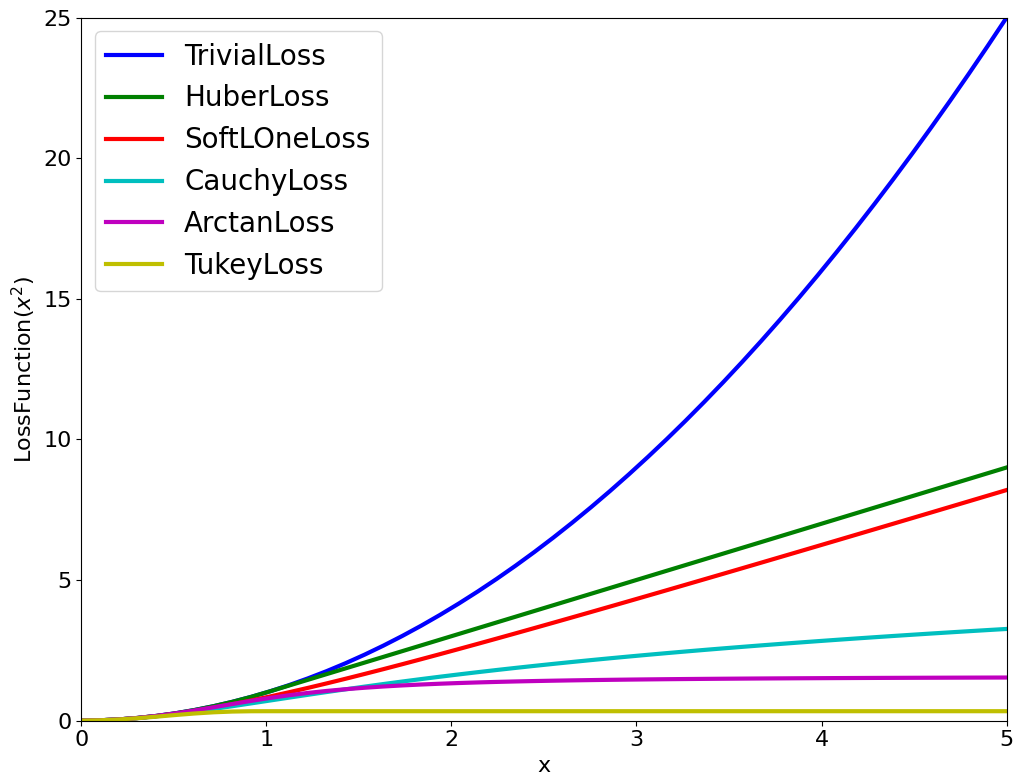
\includegraphics[width=0.5\textwidth]{images/C9_5.png}
    \caption{Robust loss functions: the trivial (squared) loss grows quadratically, the robust ones grow much more slowly}
\end{figure}

\subsection{Optimization on manifolds}
Suppose we want to estimate a \textbf{rotation} $R \in SO(3)$, e.g.\ the one that best aligns two sets of points:
\[
\min_R \sum_i \left\| y_i - R\, x_i \right\|_2^2
\]
Euler angles suffer from singularities, so we prefer quaternions or $3\times3$ matrices.
However, these representations are \textbf{over-parameterized}: a rotation has 3 degrees of freedom, while a matrix has 9 parameters and a quaternion 4.
They also have \textbf{constraints} ($R^T R = I$, $\|q\| = 1$) that make them describe the same underlying three-dimensional rotation manifold.

Moreover, to solve the problem we have to linearize it, but for rotation matrices and quaternions the operator $+$ is \textbf{not well defined}:
\[
\min_R \sum_i \left\| y_i - R\, x_i \right\|_2^2 \;\approx\; \min_{\Delta R} \sum_i \left\| y_i - (R + \Delta R)\, x_i \right\|_2^2
\]
In general, if $R$ is a rotation matrix (or a unit quaternion), $R + \Delta R$ is \textbf{not} a rotation matrix (or a unit quaternion) anymore.

\subsubsection{Manifolds and the exponential map}
\noindent\begin{minipage}[c]{0.6\textwidth}
A \textbf{manifold} is a topological space that can be \textbf{locally approximated} by a Euclidean space near each point.
For 3D rotations, the manifold is:
\[
SO(3) = \{ X \in \mathbb{R}^{3\times3} \mid \det X = 1,\ X^T X = I \}
\]
or, with quaternions:
\[
SO(3) = \{ q \in \mathbb{R}^4 \mid \|q\| = 1 \}
\]
\end{minipage}\hfill
\begin{minipage}[c]{0.35\textwidth}
    \centering
    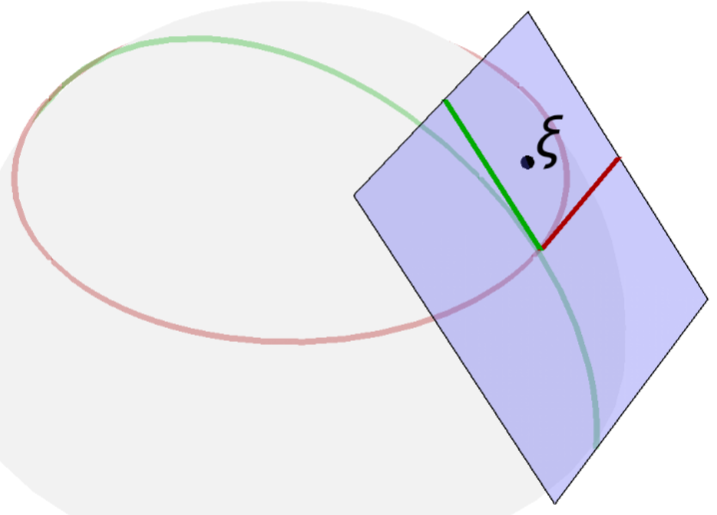
\includegraphics[width=\linewidth]{images/C9_6.png}
    \captionof{figure}{A manifold and its tangent plane}
\end{minipage}

\vspace{6pt}The \textbf{exponential map} $\exp(\cdot)$ is a function that maps a movement in the \textbf{tangent plane} to a movement on the manifold.
Since the tangent plane is a Euclidean space, we can compute the optimal update $\xi \in \mathbb{R}^3$ there (with the usual least squares), map it onto the manifold with the exponential map, and apply it to $R$:
\[
\min_{R \in SO(3)} \sum_i \left\| y_i - R\, x_i \right\|_2^2 \;\approx\; \min_{\xi \in \mathbb{R}^3} \sum_i \left\| y_i - (R \boxplus \xi)\, x_i \right\|_2^2 = \min_{\xi \in \mathbb{R}^3} \sum_i \left\| y_i - R\, \exp(\xi)\, x_i \right\|_2^2
\]
The operator $\boxplus$ is the \textbf{retraction}: the generalization of $+$ on a manifold.
In this way the update has exactly 3 parameters, and the result is always a valid rotation.

\subsubsection{Exponential map in SO(3)}
The exponential map in $SO(3)$ is given by the \textbf{Rodrigues formula}:
\[
\exp(\xi) = I + \frac{\sin\theta}{\theta}\, [\xi]_\times + \frac{1 - \cos\theta}{\theta^2}\, [\xi]_\times^2, \qquad \theta = \|\xi\|
\]
where $\xi$ is the rotation axis scaled by the rotation angle $\theta$, and $[\xi]_\times$ is its skew-symmetric matrix.
Its Jacobian, needed to linearize the residuals, is:
\[
J(\xi) = I - \frac{1 - \cos\theta}{\theta^2}\, [\xi]_\times + \frac{\theta - \sin\theta}{\theta^3}\, [\xi]_\times^2
\]

\begin{examplebox}[Optimization on a manifold in SO(2)]
\noindent\begin{minipage}[c]{0.55\linewidth}
In 2D, the rotations are the unit vectors, $SO(2) = \{ x \in \mathbb{R}^2 \mid \|x\| = 1 \}$, so the manifold is a \textbf{circle}.
Starting from $x_0$, we compute the update $\xi$ on the tangent line at $x_0$ (a Euclidean space), and the exponential map wraps it onto the circle:
\[
x_1 = x_0 \boxplus \xi
\]
The new point is still on the circle, i.e.\ still a valid rotation, which would not happen with $x_0 + \xi$.
\end{minipage}\hfill
\begin{minipage}[c]{0.4\linewidth}
    \centering
    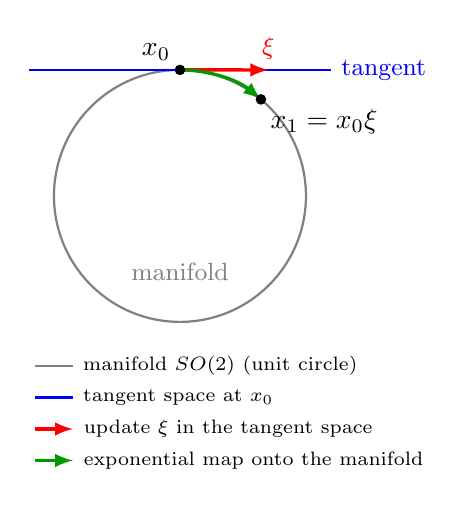
\begin{tikzpicture}[scale=1.6, >=latex]
        \draw[thick, gray] (0,0) circle (1);
        \coordinate (x0) at (90:1);
        \draw[thick, blue] (-1.2,1) -- (1.2,1) node[right, font=\small] {tangent};
        \draw[->, very thick, red] (x0) -- (0.7,1) node[above, font=\small] {$\xi$};
        \draw[->, very thick, green!60!black] (x0) arc (90:50:1);
        \fill (x0) circle (1.2pt) node[above left] {$x_0$};
        \fill (50:1) circle (1.2pt) node[below right] {$x_1 = x_0 \boxplus \xi$};
        \node[gray, font=\small] at (0,-0.6) {manifold};
        % legend
        \begin{scope}[shift={(-1.15,-1.35)}, font=\scriptsize]
            \draw[thick, gray] (0,0) -- (0.3,0) node[right, black] {manifold $SO(2)$ (unit circle)};
            \draw[thick, blue] (0,-0.25) -- (0.3,-0.25) node[right, black] {tangent space at $x_0$};
            \draw[->, very thick, red] (0,-0.5) -- (0.3,-0.5) node[right, black] {update $\xi$ in the tangent space};
            \draw[->, very thick, green!60!black] (0,-0.75) -- (0.3,-0.75) node[right, black] {exponential map onto the manifold};
        \end{scope}
    \end{tikzpicture}
\end{minipage}
\end{examplebox}

The next question is: how can we use NLLS for the \textbf{3D reconstruction} with cameras?
